\section{Differenzstufe}
In diesem Versuchsteil soll der Stromspiegel aus Versuch 1 als Stromquelle f\"ur eine
Differenzstufe verwendet werden. Es wird der Arbeitspunkt vermessen sowie die
Gleichtaktansteuerung untersucht.
Beachten Sie, dass f\"ur die Eingangstransistoren der Differenzstufe der Transistor
vom Typ BS170 verwendet wird.
\subsection{Experimentelle Durchf\"uhrung}
Die Schaltung aus Versuch 1 wurde mit zwei Widerst\"anden und zwei
Transistoren erg\"anzt des Weiteren wurde an beide Eing\"ange (U$_{ein}$ und 
$_{aus}$) eine Spannung angelegt. Zun\"achst wurde der Arbeitspunkt bestimmt,
dazu wurde die Eingangsspannung auf 0V gelegt. Anschlie\ss end wurde die
differentielle
Ausgangsspannung bestimmt und zum Schluss der Gleichtakteingangsspannungs-
bereich vermessen.
\begin{figure}[!ht]
\begin{center}
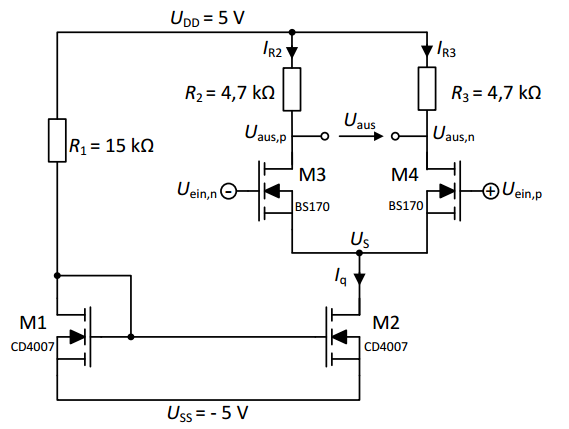
\includegraphics[scale=0.8]{Differenzstufe}
\end{center}
\end{figure}
\clearpage
\subsection{Ergebnisse und Diskussion}
\begin{figure}[!h]
\begin{center}

\includegraphics[scale=0.8]{Text}
\end{center}
\end{figure}
\begin{figure}[!ht]
\begin{center}
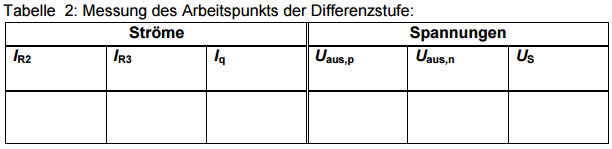
\includegraphics[scale=0.8]{Tabelle2}
\end{center}
\end{figure}
\begin{figure}[!ht]
\begin{center}
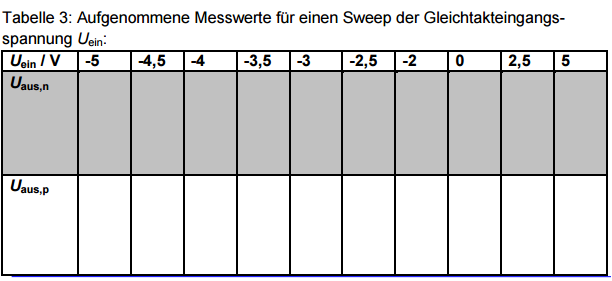
\includegraphics[scale=0.8]{Tabelle3}
\end{center}
\end{figure}
\begin{figure}[!h]
\begin{center}

\includegraphics[scale=0.8]{Text}
\end{center}
\end{figure}
\begin{figure}[!ht]
\begin{center}
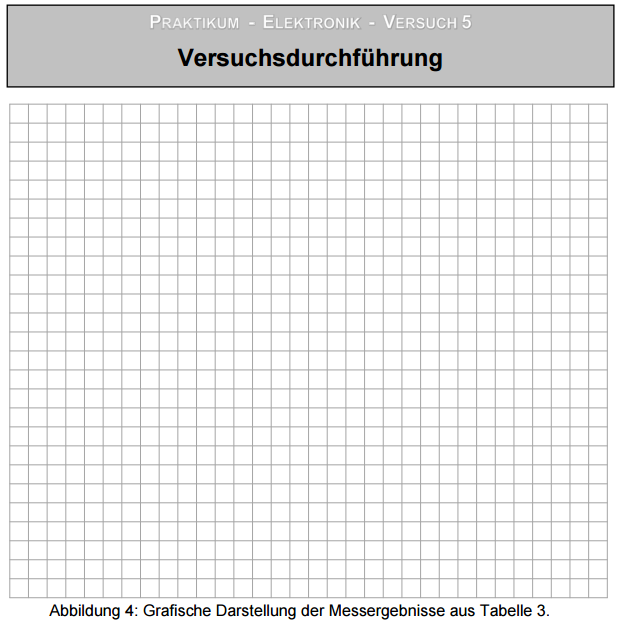
\includegraphics[scale=0.8]{Graph2}
\end{center}
\end{figure}
\clearpage
